\clearpage
% Generated by build_lifetime_timeline.py; do not hand-edit.
\newcommand{\timelinePeakAge}{0.7103}
\newcommand{\timelinePeakHe}{0.1003}
\newcommand{\timelineConvectionAge}{3.546}
\newcommand{\timelineConvectionX}{0.1751}
\newcommand{\timelineLastAge}{3.89}
\newcommand{\timelineLastX}{0.0008157}
\newcommand{\timelineLastTeff}{5546}
\newcommand{\timelineLastConvectivePercent}{2.565}
\newcommand{\timelineHydrogenCrossAge}{3.884}
\newcommand{\timelineHydrogenCrossWidthMyr}{22.72}
\newcommand{\timelineLastMean}{129.7}
\newcommand{\timelineLastLow}{128}
\newcommand{\timelineLastHigh}{132.1}

\section{Lifetime timeline}
\label{sec:lifetime}
The timeline combines the calculated hydrogen-burning track with the later
physical stages to be evaluated. Numerical ages labelled Ember come from the
track plotted in this paper. Formation precedes its age zero; subsequent
cooling ages have not yet been calculated. Environmental events and material
transitions can overlap, so their order is conditional. Disappearance means
the loss of the baryonic remnant, with energy carried away by decay products.

\subsection{Formation and hydrogen burning}
{\small\renewcommand{\arraystretch}{1.17}
\begin{tabular}{@{}>{\raggedright\arraybackslash}p{0.14\textwidth}
 >{\raggedright\arraybackslash}p{0.24\textwidth}
 >{\raggedright\arraybackslash}p{0.57\textwidth}@{}}
\toprule
Age or condition & Event & Physical description and basis \\\midrule
Before $t=0$ & Formation and accretion &
Cloud collapse assembles the protostar. Accretion, a disk and any outflows
set its initial mass, entropy and angular momentum. These stages are outside
the present fixed-mass calculation. \\[4pt]
Before $t=0$ & Deuterium burning and contraction &
The young object contracts toward sustained hydrogen burning; deuterium is
consumed, and lithium is depleted as the interior heats. Low-mass
pre-main-sequence models supply the comparison, rather than an Ember
formation age \cite{baraffe15}. \\[4pt]
$t=0$ & Fully convective hydrogen-burning model &
Ember begins with $X=0.7$, $Z=0.02$, $R=0.1259\Rs$ and
$T_{\rm eff}=2766$ K. The pp chain converts hydrogen to helium while
convection mixes the star. \\[4pt]
$\timelinePeakAge\Tyr$ & Maximum $^3$He abundance &
The calculated central $^3$He mass fraction reaches $\timelinePeakHe$ and
then decreases as its destruction catches up with its production.
LBA97 gives 0.0995 at $1.38\Tyr$. \\[4pt]
$\timelineConvectionAge\Tyr$ & Loss of full convection &
The first saved Ember structure with a nonconvective region has central
$X=\timelineConvectionX$. This does not alone date formation of a
central radiative core. LBA97 reports its central radiative core at
$5.742\Tyr$ and $X=0.16$. \\[4pt]
$3.560\Tyr$ & Separate core and envelope composition &
The calculated convective mass fraction is 0.6277. Central $X=0.1518$
differs from surface $X=0.1747$; whole-star mixing has ended. \\[4pt]
$\timelineHydrogenCrossAge\Tyr$ and onward & Central hydrogen depletion &
Central $X$ crosses $10^{-3}$ within a \timelineHydrogenCrossWidthMyr-million-year
bracket of accepted models. Crossings of $10^{-4}$ and $10^{-5}$ remain to be
calculated. Track the envelope fuel and burning outside the depleted center. \\[4pt]
$\timelineLastAge\Tyr$ & Endpoint of the plotted track &
$T_{\rm eff}=\timelineLastTeff$ K and central $X=\timelineLastX$.
Conduction and radiation carry heat through the core; the convective envelope
contains \timelineLastConvectivePercent\% of the mass.
Hydrogen burning still dominates luminosity. \\[4pt]
Age to be calculated & Turn toward white-dwarf cooling &
Track the maximum surface temperature and the change to sustained cooling.
LBA97 reaches 5807 K; this is a comparison value, not an imposed Ember turn.
The low mass leads toward a helium remnant without normal core helium burning. \\
\bottomrule
\end{tabular}}

\clearpage
\subsection{Cooling and environmental exposure}
These stages are identified by local conditions or their effect on the energy
balance. A surface temperature of 100 K is an intermediate milestone; it
does not imply a 100 K core. The calculation will compare the following
processes before assigning their event ages.

{\small\renewcommand{\arraystretch}{1.16}
\begin{tabular}{@{}>{\raggedright\arraybackslash}p{0.14\textwidth}
 >{\raggedright\arraybackslash}p{0.24\textwidth}
 >{\raggedright\arraybackslash}p{0.57\textwidth}@{}}
\toprule
Condition & Event & Physical description and calculation \\\midrule
Declining nuclear power & Residual hydrogen burning fades &
Record nuclear heating below 10\%, 1\% and 0.1\% of photon luminosity,
including any later recovery. Retain the envelope fuel supply and thermal
energy rather than assuming an immediately passive remnant. \\[4pt]
Transport competes with evolution & Diffusion and separation &
Hydrogen can collect at the surface while heavier species settle. The
atmosphere's composition follows transport and mixing; a helium core does
not imply a helium atmosphere. \\[4pt]
Envelope cools & Molecules, grains and dense atmospheres &
Follow molecular absorption, collision-induced absorption, scattering,
condensation and settling where the local conditions permit them. Couple
opacity to composition and energy transport \cite{chabrier00,blouin18}. \\[4pt]
Interior reaches a phase boundary & Crystallization and chemical separation &
Evaluate helium and mixture phase equilibria, latent heat, separation energy
and solid heat capacity. The front's progress is determined by density and
core temperature, not one assigned surface temperature \cite{baiko22}. \\[4pt]
Convection reaches deeper layers & Envelope and core become thermally coupled &
Determine whether and when the convective envelope reaches the nearly
isothermal interior, changing the relation between stored heat and luminosity.
Its order relative to crystallization is to be calculated. \\[4pt]
$T_{\rm eff}=1000$, 500, 100 K & Cold-remnant milestones &
Record ages, core temperature, radius, composition, solid fraction and power
sources on the cooling branch. Below 100 K, continue with the appropriate
solid and partly neutral matter description. \\[4pt]
Including ages $\gtrsim10^{14}$ yr & Changing environment and accretion &
Compare retained and ejected objects in evolving stellar and dark-matter
environments. Gas, debris and interstellar solid objects provide conditional
accretion and heating; no unique late encounter rate is assumed. \\[4pt]
Close passages & Tidal heating, capture or collision &
For surviving unbound WD pairs, distinguish heat from spin and persistent
oscillations. Couple an encounter survey to waiting-time distributions and
cooling after each pulse; captures and collisions form separate outcomes. \\[4pt]
Allowed particle interactions & Dark-matter heating &
Compare capture, thermalization, evaporation and possible annihilation with
the photon luminosity. Include no annihilation heating as an alternative;
crystallization can change thermalization \cite{bell24}. \\[4pt]
Nuclear times become competitive & Density-driven fusion &
Estimate pycnuclear and impurity reactions against cooling and decay times,
using the actual helium-rich composition. Carbon-burning results do not
directly determine helium-remnant rates \cite{gasques05}. \\
\bottomrule
\end{tabular}}

\clearpage
\subsection{Decay and disappearance: conditional branches}
Proton decay has not been detected. The Super-Kamiokande limit for
$p\rightarrow e^+\pi^0$ is a partial lifetime
$\tau_p/B>2.4\times10^{34}$ yr at 90\% confidence \cite{takenaka20}.
Baryogenesis does not itself require ordinary proton decay; leptogenesis
provides a counterexample \cite{fukugita86}.

Virtual-black-hole interactions supply another possible decay channel. A
Planck-scale estimate is $\tau_p\sim10^{45}$ yr, with rate set by the assumed
quantum-gravity interaction \cite{adams01}. This differs from collective
tunneling of stellar matter through its degeneracy barrier, which can be far
more suppressed \cite{adams98}. We therefore consider finite-lifetime
scenarios and a stable-baryon branch rather than assigning one disappearance
date. The assumed channel must specify which bound and free nucleons decay.

{\small\renewcommand{\arraystretch}{1.17}
\begin{tabular}{@{}>{\raggedright\arraybackslash}p{0.14\textwidth}
 >{\raggedright\arraybackslash}p{0.24\textwidth}
 >{\raggedright\arraybackslash}p{0.57\textwidth}@{}}
\toprule
Condition & Event & Physical description and calculation \\\midrule
Decay heating exceeds other sources & Decay-supported luminosity &
Compare deposited decay energy with cooling and environmental power. This
can occur long before a substantial fraction of the mass is lost. Escape
fractions depend on decay products and the evolving column density. \\[4pt]
Accumulated decays & Composition changes and mass loss &
Track baryonic mass, nuclear daughter products, subsequent decays and reaction
energy. Begin with coarse composition groups and refine only where they
change pressure, retained heat or phase order. \\[4pt]
Pressure support changes & Loss of degeneracy &
Follow the transition from a degenerate remnant to matter whose structure
depends on atomic and molecular forces. Recalculate the mass-radius relation;
do not impose a transition mass from a different composition. \\[4pt]
Columns become small & Decay products and thermal radiation escape &
Separate transparency to energetic decay products from transparency at thermal
wavelengths. Decreasing energy retention changes luminosity and temperature;
an optically thin object need not radiate as a blackbody. \\[4pt]
Binding becomes insufficient & End of the bound remnant &
Allow fragmentation or dispersal if the material and energy balance require it.
This is distinct from decay of every formerly associated baryon. Accretion,
capture or collision can interrupt the isolated path at other stages. \\[4pt]
Few baryons remain & Discrete survival and final decay &
Replace a continuous mass variable with particle survival probabilities.
Specify any stable products. If all original baryons have finite lifetimes,
their last decay is a random event; an exponential mean never reaches zero
at a finite time. \\[4pt]
Stable-baryon alternative & No decay-imposed endpoint &
Continue cooling, nuclear and environmental alternatives without assigning a
proton-decay date. Any gravitational destruction channel requires its own
assumptions and rate. \\
\bottomrule
\end{tabular}}

The degree of physical detail follows the quantity being predicted. Resolved
atmospheres and interior transport determine the stellar track and cooling
ages. At more uncertain stages, thermal balances, encounter distributions
and conditional decay models are sufficient unless additional structure changes
the result. Numerical errors must still be smaller than the signal of interest,
especially for weak tidal heating. Successive descriptions will be compared
where both apply, preserving mass, composition and stored energy.

\clearpage
\subsection{A reference clock for the decay era}
A useful analytic comparison assumes that every baryon has the same constant,
independent mean lifetime $\tau_B$, with no accretion or stable daughter baryons.
Let $t_d$ measure elapsed time from the start of this comparison. Then
\begin{equation}
 \langle M_B(t_d)\rangle=M_{B,0}e^{-t_d/\tau_B},\qquad
 L_{\rm heat}=f_{\rm dep}(t_d)\frac{\langle M_B\rangle c^2}{\tau_B}.
\end{equation}
The second expression treats baryon mass as the available rest energy;
a physical channel also accounts for daughter masses and nuclear binding.
The deposited fraction $f_{\rm dep}$ is allowed to evolve. This is a reference
mass and energy model, not a resolved calculation of the late atmosphere.

\begin{center}\small
\begin{tabular}{@{}lr@{}}\toprule
Expected initial baryonic mass lost & $t_d/\tau_B$ \\\midrule
50\% & 0.6931 \\
90\% & 2.303 \\
99\% & 4.605 \\
99.99\% & 9.210 \\\bottomrule
\end{tabular}\end{center}

For $N_0$ independently decaying baryons the last-event distribution is
\begin{equation}
 \Pr(t_{\rm last}\leq t_d)=\left(1-e^{-t_d/\tau_B}\right)^{N_0},\qquad
 \langle t_{\rm last}\rangle=\tau_B H_{N_0},
\end{equation}
where $H_N=\sum_{k=1}^{N}1/k$. For an initial baryonic mass $0.1\Ms$,
$N_0\simeq1.2\times10^{56}$. The mean last decay occurs near
$\timelineLastMean\,\tau_B$, with a central 90\% interval from
$\timelineLastLow$ to $\timelineLastHigh\,\tau_B$.
This follows all tagged original baryons, including any dispersed material;
it does not date the survival of a bound star. Correlated processes,
composition-dependent lifetimes and stable products change this reference.

\begin{figure}[H]\centering
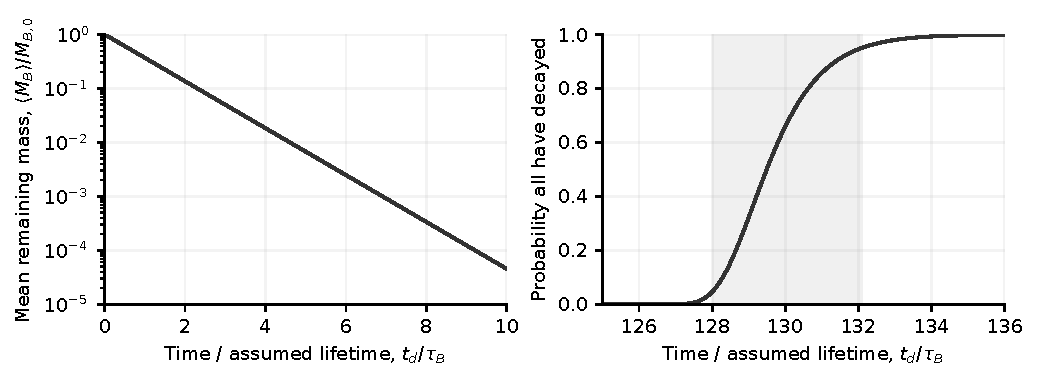
\includegraphics[width=\textwidth]{lifetime_decay_reference.pdf}
\caption{Conditional decay reference for an initially $0.1\Ms$ baryon
population with one independent lifetime. Left: expected remaining mass.
Right: probability that all original baryons have decayed; shading marks
the central 90\% last-event interval. The two time ranges differ. These
curves are analytic consequences of the stated assumptions, not an
extrapolation of the computed Ember track.}
\end{figure}
